\documentclass[oneside,11pt,a4paper,]{book}
\usepackage{lmodern}
\usepackage{amssymb,amsmath}
\usepackage{ifxetex,ifluatex}
\usepackage{fixltx2e} % provides \textsubscript
\ifnum 0\ifxetex 1\fi\ifluatex 1\fi=0 % if pdftex
  \usepackage[T1]{fontenc}
  \usepackage[utf8]{inputenc}
\else % if luatex or xelatex
  \ifxetex
    \usepackage{mathspec}
    \usepackage{xltxtra,xunicode}
  \else
    \usepackage{fontspec}
  \fi
  \defaultfontfeatures{Mapping=tex-text,Scale=MatchLowercase}
  \newcommand{\euro}{€}
    \setmainfont{Lato}
    \setmonofont[Mapping=tex-ansi]{Menlo}
\fi
% use upquote if available, for straight quotes in verbatim environments
\IfFileExists{upquote.sty}{\usepackage{upquote}}{}
% use microtype if available
\IfFileExists{microtype.sty}{%
\usepackage{microtype}
\UseMicrotypeSet[protrusion]{basicmath} % disable protrusion for tt fonts
}{}
\usepackage{color}
\usepackage{fancyvrb}
\newcommand{\VerbBar}{|}
\newcommand{\VERB}{\Verb[commandchars=\\\{\}]}
\DefineVerbatimEnvironment{Highlighting}{Verbatim}{commandchars=\\\{\}}
% Add ',fontsize=\small' for more characters per line
\usepackage{framed}
\definecolor{shadecolor}{RGB}{248,248,248}
\newenvironment{Shaded}{\begin{snugshade}}{\end{snugshade}}
\newcommand{\KeywordTok}[1]{\textcolor[rgb]{0.13,0.29,0.53}{\textbf{{#1}}}}
\newcommand{\DataTypeTok}[1]{\textcolor[rgb]{0.13,0.29,0.53}{{#1}}}
\newcommand{\DecValTok}[1]{\textcolor[rgb]{0.00,0.00,0.81}{{#1}}}
\newcommand{\BaseNTok}[1]{\textcolor[rgb]{0.00,0.00,0.81}{{#1}}}
\newcommand{\FloatTok}[1]{\textcolor[rgb]{0.00,0.00,0.81}{{#1}}}
\newcommand{\CharTok}[1]{\textcolor[rgb]{0.31,0.60,0.02}{{#1}}}
\newcommand{\StringTok}[1]{\textcolor[rgb]{0.31,0.60,0.02}{{#1}}}
\newcommand{\CommentTok}[1]{\textcolor[rgb]{0.56,0.35,0.01}{\textit{{#1}}}}
\newcommand{\OtherTok}[1]{\textcolor[rgb]{0.56,0.35,0.01}{{#1}}}
\newcommand{\AlertTok}[1]{\textcolor[rgb]{0.94,0.16,0.16}{{#1}}}
\newcommand{\FunctionTok}[1]{\textcolor[rgb]{0.00,0.00,0.00}{{#1}}}
\newcommand{\RegionMarkerTok}[1]{{#1}}
\newcommand{\ErrorTok}[1]{\textbf{{#1}}}
\newcommand{\NormalTok}[1]{{#1}}
\usepackage{longtable,booktabs}
\usepackage{graphicx}
\makeatletter
\def\maxwidth{\ifdim\Gin@nat@width>\linewidth\linewidth\else\Gin@nat@width\fi}
\def\maxheight{\ifdim\Gin@nat@height>\textheight\textheight\else\Gin@nat@height\fi}
\makeatother
% Scale images if necessary, so that they will not overflow the page
% margins by default, and it is still possible to overwrite the defaults
% using explicit options in \includegraphics[width, height, ...]{}
\setkeys{Gin}{width=\maxwidth,height=\maxheight,keepaspectratio}
\ifxetex
  \usepackage[setpagesize=false, % page size defined by xetex
              unicode=false, % unicode breaks when used with xetex
              xetex]{hyperref}
\else
  \usepackage[unicode=true]{hyperref}
\fi
\hypersetup{breaklinks=true,
            bookmarks=true,
            pdfauthor={Dave Gurnell},
            pdftitle={Essential Play},
            colorlinks=true,
            citecolor=blue,
            urlcolor=blue,
            linkcolor=magenta,
            pdfborder={0 0 0}}
\urlstyle{same}  % don't use monospace font for urls
\setlength{\parindent}{0pt}
\setlength{\parskip}{6pt plus 2pt minus 1pt}
\setlength{\emergencystretch}{3em}  % prevent overfull lines
\setcounter{secnumdepth}{5}

\title{Essential Play}
\author{Dave Gurnell}
\date{}

\usepackage[xcolor]{mdframed}
\newmdenv[%
  topline=false,bottomline=false,leftline=false,rightline=false,linewidth=0,
  leftmargin=0,rightmargin=0,innertopmargin=1em,innerbottommargin=1em,
  frametitlebelowskip=1em,
  backgroundcolor=blue!5,
  frametitle=Tip]{InfoCallout}
\newmdenv[%
  topline=false,bottomline=false,leftline=false,rightline=false,linewidth=0,
  leftmargin=0,rightmargin=0,innertopmargin=1em,innerbottommargin=1em,
  frametitlebelowskip=1em,
  backgroundcolor=yellow!10,
  frametitle=Advanced]{WarningCallout}
\newmdenv[%
  topline=false,bottomline=false,leftline=false,rightline=false,linewidth=0,
  leftmargin=0,rightmargin=0,innertopmargin=1em,innerbottommargin=1em,
  frametitlebelowskip=1em,
  backgroundcolor=red!5,
  frametitle=Warning]{DangerCallout}

\DefineVerbatimEnvironment{Highlighting}{Verbatim}{commandchars=\\\{\},fontsize=\small}

\begin{document}
\maketitle

{
\hypersetup{linkcolor=black}
\setcounter{tocdepth}{4}
\tableofcontents
}
\pagebreak

\chapter{Foreword}\label{foreword}

This course is aimed at beginner-to-intermediate Scala developers who
want to get started using the \href{http://playframework.com}{Play 2}
web framework. By the end of the course we will have a solid foundation
in each of the main libraries Play provides for building sites and
services:

\begin{itemize}
\itemsep1pt\parskip0pt\parsep0pt
\item
  Routing, controllers, and actions
\item
  Manipulating requests and responses
\item
  Generating HTML
\item
  Parsing and validating form data
\item
  Reading and writing JSON
\item
  Asynchronous request handling
\item
  Calling external web services
\end{itemize}

As coursework we will build a simple chat application from the ground
up. We will start with a very basic web site and end up building a
complete service-oriented architecture with each concern separated out
to a separate microservice.

The material presented focuses on Play version 2.3, although the
approaches introduced are generally applicable to Play 2.2+.

\chapter{The Basics}\label{chapter-basics}

In this chapter we will introduce five fundamental concepts used to
process web requests in Play: \emph{actions}, \emph{controllers},
\emph{routes}, \emph{requests}, and \emph{results}. With these concepts
we will be able to read incoming HTTP requests, pass them to the correct
module of application code, extract appropriate information, and send a
response back to the client.

\section{Actions, Controllers, and
Routes}\label{actions-controllers-and-routes}

We create Play web applications from \emph{actions}, \emph{controllers},
and \emph{routes}. In this section we will see what each part does and
how to wire them together.

\subsection{Hello, World!}\label{hello-world}

\emph{Actions} are objects that handle web requests. They have an
\texttt{apply} method that accepts a
\href{https://www.playframework.com/documentation/2.3.x/api/scala/index.html\#play.api.mvc.Request}{play.api.mvc.Request}
and returns a
\href{https://www.playframework.com/documentation/2.3.x/api/scala/index.html\#play.api.mvc.Result}{play.api.mvc.Result}

\begin{Shaded}
\begin{Highlighting}[]
\NormalTok{Action \{ request =>}
  \FunctionTok{Ok}\NormalTok{(}\StringTok{"Hello, world!"}\NormalTok{)}
\NormalTok{\}}
\end{Highlighting}
\end{Shaded}

We package actions inside \texttt{Controllers}. These are singleton
objects that contain action-producing methods:

\begin{Shaded}
\begin{Highlighting}[]
\KeywordTok{package} \NormalTok{controllers}

\KeywordTok{import} \NormalTok{play.}\FunctionTok{api}\NormalTok{.}\FunctionTok{mvc}\NormalTok{.\{ Action, Controller \}}

\KeywordTok{object} \NormalTok{HelloController }\KeywordTok{extends} \NormalTok{Controller \{}
  \KeywordTok{def} \NormalTok{hello = Action \{ request =>}
    \FunctionTok{Ok}\NormalTok{(}\StringTok{"Hello, world!"}\NormalTok{)}
  \NormalTok{\}}

  \KeywordTok{def} \FunctionTok{helloTo}\NormalTok{(name: String) = Action \{ request =>}
    \FunctionTok{Ok}\NormalTok{(s}\StringTok{"Hello, $name!"}\NormalTok{)}
  \NormalTok{\}}
\NormalTok{\}}
\end{Highlighting}
\end{Shaded}

We use \emph{routes} to dispatch incoming requests to \texttt{Actions}.
They choose \texttt{Actions} based on the \emph{HTTP method} and
\emph{path} of the request. We write routes in a Play-specific DSL that
is compiled to Scala by SBT -- we'll learn more about this DSL in the
next section:

\begin{Shaded}
\begin{Highlighting}[]
\KeywordTok{GET} \NormalTok{/      controllers.HelloController.hello}
\KeywordTok{GET} \NormalTok{/:name controllers.HelloController.helloTo(name: String)}
\end{Highlighting}
\end{Shaded}

By convention we place controllers in the \texttt{controllers} package
in the \texttt{app/controllers} folder, and routes in a
\texttt{conf/routes} configuration file. This is the structure of a
basic Play application:

\begin{Shaded}
\begin{Highlighting}[]
\NormalTok{myProject}\KeywordTok{/}
  \NormalTok{build}\KeywordTok{.}\NormalTok{sbt                 }\CommentTok{# SBT project configuration}
  \NormalTok{project}\KeywordTok{/}
    \NormalTok{plugins}\KeywordTok{.}\NormalTok{sbt             }\CommentTok{# SBT plugin configuration}
  \NormalTok{app}\KeywordTok{/}
    \NormalTok{controllers}\KeywordTok{/}            \CommentTok{# Controllers and actions go here}
      \NormalTok{HelloController}\KeywordTok{.}\NormalTok{scala }\CommentTok{#}
  \NormalTok{conf}\KeywordTok{/}
    \NormalTok{routes                  }\CommentTok{# Routes go here}
\end{Highlighting}
\end{Shaded}

\subsection{The Anatomy of a
Controller}\label{the-anatomy-of-a-controller}

Let's take a closer look at the controller in the example above. The
code in use comes from two places:

\begin{itemize}
\itemsep1pt\parskip0pt\parsep0pt
\item
  the
  \href{https://www.playframework.com/documentation/2.3.x/api/scala/index.html\#play.api.mvc.package}{play.api.mvc}
  package;
\item
  the
  \href{https://www.playframework.com/documentation/2.3.x/api/scala/index.html\#play.api.mvc.Controller}{play.api.mvc.Controller}
  trait (via inheritance).
\end{itemize}

The controller, called \texttt{HelloController}, is a subtype of
\href{https://www.playframework.com/documentation/2.3.x/api/scala/index.html\#play.api.mvc.Controller}{play.api.mvc.Controller}.
It defines two \texttt{Action}-producing methods, \texttt{hello} and
\texttt{helloTo}. Our routes specify which of these methods to call when
a request comes in.

Note that \texttt{Actions} and \texttt{Controllers} have different
lifetimes. \texttt{Controllers} are created when our application boots
and persist until it shuts down. \texttt{Actions} are created by method
calls and only live long enough to handle a single \texttt{Request}.
Play passes the parameters from our routes to \emph{the method that
creates the \texttt{Action}}, not to the action itself.

Each of the example \texttt{Actions} creates an \texttt{Ok} response
containing a simple message. \texttt{Ok} is a helper object inherited
from \texttt{Controller}. It has an \texttt{apply} method that creates
\texttt{Results} with HTTP status 200. The actual return type of
\texttt{Ok.apply} is
\href{https://www.playframework.com/documentation/2.3.x/api/scala/index.html\#play.api.mvc.Result}{play.api.mvc.Result}.

Play uses the type of the argument to \texttt{Ok.apply} to determine the
\texttt{Content-Type} of the \texttt{Result}. The \texttt{String}
arguments in the example create a \texttt{Results} of type
\texttt{text/plain}. Later on we'll see how to customise this behaviour
and create results of different types.

\subsection{Take Home Points}\label{take-home-points}

We create Play web applications from \texttt{Actions},
\texttt{Controllers}, and \emph{routes}.

\begin{itemize}
\item
  \texttt{Actions} are functions from \texttt{Requests} to
  \texttt{Results};
\item
  \texttt{Controllers} are collections of action-producing methods;
\item
  \textbf{Routes} map incoming \texttt{Requests} to
  \texttt{Action}-producing method calls on our \texttt{Controllers}.
\end{itemize}

We typically place controllers in a \texttt{Controllers} package in the
\texttt{app/controllers} folder. Routes go in the \texttt{conf/routes}
file (no filename extension).

In the next section we will take a closer look at routes.

\section{Routes in Depth}\label{routes-in-depth}

The previous section introduced actions, controllers, and routes.
Actions and controllers are standard Scala code, but routes are
something new and specific to Play.

We define Play routes using a special DSL that compiles to Scala code.
The DSL provides both a convenient way of mapping URIs to method calls,
and a way of mapping method calls \emph{back} to URIs. In this section
we will take a deeper look at Play's routing DSL, including the various
ways we can extract parameters from URIs.

\subsection{Path Parameters}\label{path-parameters}

Routes associate \emph{URI patterns} with \emph{action-producing method
calls}. We can specify \emph{parameters} to extract from the URI and
pass to our controllers. Here are some examples:

\begin{Shaded}
\begin{Highlighting}[]
\CommentTok{# Fixed route (no parameters):}
\NormalTok{GET }\KeywordTok{/}\NormalTok{hello controllers}\KeywordTok{.}\NormalTok{HelloController}\KeywordTok{.}\NormalTok{hello}

\CommentTok{# Single parameter:}
\NormalTok{GET }\StringTok{/hello/}\KeywordTok{:}\NormalTok{name controllers}\KeywordTok{.}\NormalTok{HelloController}\KeywordTok{.}\NormalTok{helloTo}\KeywordTok{(}\NormalTok{name}\KeywordTok{:} \OtherTok{String}\KeywordTok{)}

\CommentTok{# Multiple parameters:}
\NormalTok{GET }\StringTok{/send/}\KeywordTok{:}\NormalTok{msg}\StringTok{/to/}\KeywordTok{:}\NormalTok{user ↩}
  \NormalTok{controllers}\KeywordTok{.}\NormalTok{ChatController}\KeywordTok{.}\NormalTok{send}\KeywordTok{(}\NormalTok{msg}\KeywordTok{:} \OtherTok{String}\KeywordTok{,} \NormalTok{user}\KeywordTok{:} \OtherTok{String}\KeywordTok{)}

\CommentTok{# Rest-style parameter:}
\NormalTok{GET }\StringTok{/download/}\KeywordTok{*}\NormalTok{filename ↩}
  \NormalTok{controllers}\KeywordTok{.}\NormalTok{DownloadController}\KeywordTok{.}\NormalTok{file}\KeywordTok{(}\NormalTok{filename}\KeywordTok{:} \OtherTok{String}\KeywordTok{)}
\end{Highlighting}
\end{Shaded}

The first example assocates a single URL with a parameterless method.
The match must be exact -- only \texttt{GET} requests to \texttt{/hello}
will be routed. Even a trailing slash in the URI (\texttt{/hello/}) will
cause a mismatch.

The second example introduces a \emph{single-segment parameter}, written
using a leading colon (`:'). Single-segment parameters match any
continuous set of characters \emph{excluding} forward slashes (`/'). The
parameter is extracted and passed to the method call -- the rest of the
URI must match exactly.

The third example uses two single-segment parameters to extract two
parts of the URI. Again, the rest of the URI must match exactly.

The final example uses a \emph{rest-parameter}, written using a leading
asterisk ('*'). Rest-style parameters match all remaining characters in
the URI, including forward slashes.

\subsection{Matching Requests to
Routes}\label{matching-requests-to-routes}

When a request comes in, Play attempts to route it to an action. It
examines each route in turn until it finds a match. If no routes match,
it returns a 404 response.

Routes match if the HTTP method has the relevant value and the URI
matches the shape of the pattern. Play supports all eight HTTP methods:
\texttt{OPTIONS}, \texttt{GET}, \texttt{HEAD}, \texttt{POST},
\texttt{PUT}, \texttt{DELETE}, \texttt{TRACE}, and \texttt{CONNECT}:

\begin{Shaded}
\begin{Highlighting}[]
\NormalTok{GET }\KeywordTok{/}\NormalTok{hello}
  \NormalTok{➥ controllers}\KeywordTok{.}\NormalTok{HelloController}\KeywordTok{.}\NormalTok{hello}

\NormalTok{GET }\StringTok{/hello/}\NormalTok{dave}
  \NormalTok{➥ controllers}\KeywordTok{.}\NormalTok{HelloController}\KeywordTok{.}\NormalTok{helloTo}\KeywordTok{(}\StringTok{"dave"}\KeywordTok{)}

\NormalTok{GET }\StringTok{/send/}\NormalTok{hello}\StringTok{/to/}\NormalTok{dave}
  \NormalTok{➥ controllers}\KeywordTok{.}\NormalTok{ChatController}\KeywordTok{.}\NormalTok{send}\KeywordTok{(}\StringTok{"hello"}\KeywordTok{,} \StringTok{"dave"}\KeywordTok{)}

\NormalTok{GET }\StringTok{/download/}\NormalTok{path}\StringTok{/to/}\NormalTok{file}\KeywordTok{.}\NormalTok{txt}
  \NormalTok{➥ controllers}\KeywordTok{.}\NormalTok{DownloadController}\KeywordTok{.}\NormalTok{file}\KeywordTok{(}\StringTok{"path/to/file.txt"}\KeywordTok{)}

\NormalTok{GET }\StringTok{/hello/}
  \NormalTok{➥ }\DecValTok{404} \KeywordTok{(}\NormalTok{trailing slash}\KeywordTok{)}

\NormalTok{POST }\KeywordTok{/}\NormalTok{hello}
  \NormalTok{➥ }\DecValTok{404} \KeywordTok{(}\NormalTok{POST request}\KeywordTok{)}

\NormalTok{GET }\StringTok{/send/}\NormalTok{to}\KeywordTok{/}\NormalTok{dave}
  \NormalTok{➥ }\DecValTok{404} \KeywordTok{(}\NormalTok{missing path segment}\KeywordTok{)}

\NormalTok{GET }\StringTok{/send/}\NormalTok{a}\StringTok{/message/}\NormalTok{to}\KeywordTok{/}\NormalTok{dave}
  \NormalTok{➥ }\DecValTok{404} \KeywordTok{(}\NormalTok{extra path segment}\KeywordTok{)}
\end{Highlighting}
\end{Shaded}

\begin{InfoCallout}

\emph{Play Routing is Strict}

Play's strict adherance to its routing rules can sometimes be
problematic. Failing to match the URI \texttt{/hello/}, for example, may
seem overzealous. We can work around this issue easily by mapping
multiple routes to a single method call:

\begin{Shaded}
\begin{Highlighting}[]
\NormalTok{GET  }\KeywordTok{/}\NormalTok{hello  controllers}\KeywordTok{.}\NormalTok{HelloController}\KeywordTok{.}\NormalTok{hello }\CommentTok{# no trailing slash}
\NormalTok{GET  }\StringTok{/hello/} \NormalTok{controllers}\KeywordTok{.}\NormalTok{HelloController}\KeywordTok{.}\NormalTok{hello }\CommentTok{# trailing slash}
\NormalTok{POST }\StringTok{/hello/} \NormalTok{controllers}\KeywordTok{.}\NormalTok{HelloController}\KeywordTok{.}\NormalTok{hello }\CommentTok{# POST request}
\CommentTok{# and so on...}
\end{Highlighting}
\end{Shaded}

\end{InfoCallout}

\subsection{Query Parameters}\label{query-parameters}

We can specify parameters in the method-call section of a route without
declaring them in the URI. When we do this Play extracts the values from
the query string instead:

\begin{Shaded}
\begin{Highlighting}[]
\NormalTok{GET }\StringTok{/send/}\KeywordTok{:}\NormalTok{message}\StringTok{/to/}\KeywordTok{:}\NormalTok{username ↩}
  \NormalTok{controllers}\KeywordTok{.}\NormalTok{ChatController}\KeywordTok{.}\NormalTok{send}\KeywordTok{(}\NormalTok{message}\KeywordTok{:} \OtherTok{String}\KeywordTok{,} \NormalTok{username}\KeywordTok{:} \OtherTok{String}\KeywordTok{)}
\end{Highlighting}
\end{Shaded}

We sometimes want to make query string parameters optional. To do this,
we just have to define them as \texttt{Option} types. Play will pass
\texttt{Some(value)} if the URI contains the parameter and \texttt{None}
if it does not.

For example, if we have the following \texttt{Action}:

\begin{Shaded}
\begin{Highlighting}[]
\KeywordTok{object} \NormalTok{NotificationController \{}
  \KeywordTok{def} \FunctionTok{notify}\NormalTok{(username: String, message: Option[String]) =}
    \NormalTok{Action \{ request => }\CommentTok{/* ... */} \NormalTok{\}}
\NormalTok{\}}
\end{Highlighting}
\end{Shaded}

we can invoke it with the following route:

\begin{Shaded}
\begin{Highlighting}[]
\NormalTok{GET }\KeywordTok{/}\NormalTok{notify controllers}\KeywordTok{.}\NormalTok{NotificationController}\KeywordTok{.} \NormalTok{↩}
  \NormalTok{notify}\KeywordTok{(}\NormalTok{username}\KeywordTok{:} \OtherTok{String}\KeywordTok{,} \NormalTok{message}\KeywordTok{:} \NormalTok{Option}\KeywordTok{[}\OtherTok{String}\KeywordTok{])}
\end{Highlighting}
\end{Shaded}

We can mix and match required and optional query parameters as we see
fit -- in the example, \texttt{username} is required and
\texttt{message} is optional. However, \emph{path} parameters are always
required -- the following route fails to compile because the path
parameter \texttt{:message} cannot be optional:

\begin{Shaded}
\begin{Highlighting}[]
\NormalTok{GET }\StringTok{/notify/}\KeywordTok{:}\NormalTok{username}\KeywordTok{/:}\NormalTok{message controllers}\KeywordTok{.}\NormalTok{NotificationController}\KeywordTok{.} \NormalTok{↩}
  \NormalTok{notify}\KeywordTok{(}\NormalTok{username}\KeywordTok{:} \OtherTok{String}\KeywordTok{,} \NormalTok{message}\KeywordTok{:} \NormalTok{Option}\KeywordTok{[}\OtherTok{String}\KeywordTok{])}

\CommentTok{# Fails to compile with the following error:}
\CommentTok{#     [error] conf/routes:1: No path binder found for Option[String].}
\CommentTok{#     Try to implement an implicit PathBindable for this type.}
\end{Highlighting}
\end{Shaded}

\subsection{Typed Parameters}\label{typed-parameters}

We can extract path and query parameters of types other than
\texttt{String}. Play has built-in support for \texttt{Int},
\texttt{Double}, \texttt{Long}, \texttt{Boolean}, \texttt{UUID}, and
\texttt{Option} and \texttt{Seq} variants:

\begin{Shaded}
\begin{Highlighting}[]
\NormalTok{GET }\StringTok{/add/}\KeywordTok{:}\NormalTok{a}\StringTok{/to/}\KeywordTok{:}\NormalTok{b controllers}\KeywordTok{.}\NormalTok{Calculator}\KeywordTok{.}\NormalTok{add}\KeywordTok{(}\NormalTok{a}\KeywordTok{:} \NormalTok{Int}\KeywordTok{,} \NormalTok{b}\KeywordTok{:} \NormalTok{Int}\KeywordTok{)}
\end{Highlighting}
\end{Shaded}

This allows us to define \texttt{Actions} using well-typed arguments
without messy parsing code:

\begin{Shaded}
\begin{Highlighting}[]
\KeywordTok{object} \NormalTok{Calculator }\KeywordTok{extends} \NormalTok{Controller \{}
  \KeywordTok{def} \FunctionTok{add}\NormalTok{(a: Int, b: Int) = Action \{ request =>}
    \FunctionTok{Ok}\NormalTok{(s}\StringTok{"The answer is $\{a + b\}"}\NormalTok{)}
  \NormalTok{\}}
\NormalTok{\}}
\end{Highlighting}
\end{Shaded}

If Play cannot extract values of the correct type for each parameter in
a route, it returns a \emph{400 Bad Request} response to the client. It
doesn't consider any other routes lower in the file.

\begin{WarningCallout}

\emph{Custom Parameter Types}

Play parses route parameters using instances of two different \emph{type
classes}:

\begin{itemize}
\itemsep1pt\parskip0pt\parsep0pt
\item
  \href{https://www.playframework.com/documentation/2.3.x/api/scala/index.html\#play.api.mvc.PathBindable}{play.api.mvc.PathBindable}
  to extract path parameters;
\item
  \href{https://www.playframework.com/documentation/2.3.x/api/scala/index.html\#play.api.mvc.QueryStringBindable}{play.api.mvc.QueryStringBindable}
  to extract query parameters.
\end{itemize}

We can implement custom parameter types by creating implicit values
these type classes. See the linked Scaladocs for more information.

\end{WarningCallout}

\subsection{Reverse Routing}\label{reverse-routing}

\emph{Reverse routes} are objects that we can use to generate URLs from
method calls. This allows us to create URLs from type-checked program
code without having to concatenate \texttt{Strings} by hand.

Play generates reverse routes for us and places them in a
\texttt{controllers.routes} package that we can access from our Scala
code:

\begin{Shaded}
\begin{Highlighting}[]
\KeywordTok{import} \NormalTok{play.}\FunctionTok{api}\NormalTok{.}\FunctionTok{mvc}\NormalTok{.}\FunctionTok{Call}

\KeywordTok{val} \NormalTok{methodAndUri: Call = routes.}\FunctionTok{HelloController}\NormalTok{.}\FunctionTok{helloTo}\NormalTok{(}\StringTok{"dave"}\NormalTok{)}

\NormalTok{methodAndUri.}\FunctionTok{method} \CommentTok{// "GET"}
\NormalTok{methodAndUrl.}\FunctionTok{url}    \CommentTok{// "/hello/dave"}
\end{Highlighting}
\end{Shaded}

Play generates reverse routes for each controller and action referenced
in our routes file. The routes return
\href{https://www.playframework.com/documentation/2.3.x/api/scala/index.html\#play.api.mvc.Call}{play.api.mvc.Call}
objects that hold the HTTP method and URI from the route. Here is some
pseudo-code based on example above to illustrate:

\begin{Shaded}
\begin{Highlighting}[]
\KeywordTok{package} \NormalTok{routes}

\KeywordTok{import} \NormalTok{play.}\FunctionTok{api}\NormalTok{.}\FunctionTok{mvc}\NormalTok{.}\FunctionTok{Call}

\KeywordTok{object} \NormalTok{HelloController \{}
  \KeywordTok{def} \NormalTok{hello: Call =}
    \FunctionTok{Call}\NormalTok{(}\StringTok{"GET"}\NormalTok{, }\StringTok{"/hello"}\NormalTok{)}

  \KeywordTok{def} \FunctionTok{helloTo}\NormalTok{(name: String): Call =}
    \FunctionTok{Call}\NormalTok{(}\StringTok{"GET"}\NormalTok{, }\StringTok{"/hello/"} \NormalTok{+ }\FunctionTok{encodeURIComponent}\NormalTok{(name))}
\NormalTok{\}}

\KeywordTok{object} \NormalTok{ChatController \{}
  \KeywordTok{def} \FunctionTok{send}\NormalTok{(msg: String, user: String): Call =}
    \FunctionTok{Call}\NormalTok{(}\StringTok{"GET"}\NormalTok{,}
      \StringTok{"/send/"} \NormalTok{+ }\FunctionTok{encodeURIComponent}\NormalTok{(msg) +}
      \StringTok{"/to/"} \NormalTok{+ }\FunctionTok{encodeURIComponent}\NormalTok{(user))}
\NormalTok{\}}

\KeywordTok{object} \NormalTok{DownloadController \{}
  \KeywordTok{def} \FunctionTok{file}\NormalTok{(filename: String): Call =}
    \FunctionTok{Call}\NormalTok{(}\StringTok{"GET"}\NormalTok{, }\StringTok{"/download/"} \NormalTok{+ }\FunctionTok{encodeURI}\NormalTok{(filename))}
\NormalTok{\}}
\end{Highlighting}
\end{Shaded}

\subsection{Take Home Points}\label{take-home-points-1}

\emph{Routes} provide bi-directional mapping between URLs and
\texttt{Action}-producing methods within \texttt{Controllers}.

We write routes using a Play-specific DSL that compiles to Scala code.
Each route comprises an HTTP method, a URL pattern, and a corresponding
method call. Patterns can contain \emph{path} and \emph{query
parameters} that are extracted and used in the method call.

We can \emph{type} the path and query parameters in routes to simplify
the parsing code in our controllers and actions. Play supports many
types out of the box, but we can also write code to map our own types.

Play also generates \emph{reverse routes} that map method calls back to
URIs. These are placed in a synthetic \texttt{routes} package that we
can access from our Scala code.

Now we have seen what we can do with routes, let's look at the
\texttt{Request} and \texttt{Result} handling code we can write in our
actions. This will arm us with all the knowledge we need to start
dealing with HTML in the next chapter.

\section{Parsing Requests}\label{parsing-requests}

So far we have seen how to create \texttt{Actions} and map them to URIs
using \emph{routes}. In the rest of this chapter we will take a closer
look at the code we write in the actions themselves.

The first job of any \texttt{Action} is to extract data from the HTTP
request and turn it into well-typed, validated Scala values. We have
already seen how \emph{routes} allow us to extract information from the
URI. In this section we will see the other tools Play provides for the
rest of the \texttt{Request}.

Request Bodies

The most important source of request data comes from the \emph{body}.
Clients can \texttt{POST} or \texttt{PUT} data in a huge range of
formats, the most common being JSON, XML, and form data. Our first task
is to identify the content type and parse the body.

Confession time. Up to this point we've been telling a white lie about
\texttt{Request} -- it is actually a generic type,
\texttt{Request{[}A{]}}. The parameter \texttt{A} indicates the type of
body, which we can retrieve via the \texttt{body} method:

\begin{Shaded}
\begin{Highlighting}[]
\KeywordTok{def} \NormalTok{index = Action \{ request =>}
  \KeywordTok{val} \NormalTok{body: ??? = request.}\FunctionTok{body}
  \CommentTok{// ... what type is `body`? ...}
\NormalTok{\}}
\end{Highlighting}
\end{Shaded}

Play contains an number of \emph{body parsers} that we can use to parse
the request, returning a \texttt{body} of an appropriate Scala type.

So what type does \texttt{request.body} return in the examples we've
seen so far? We haven't chosen a body parser, nor have we indicated the
type of body anywhere in our code. Play \emph{cannot} know the
content-type of a request at compile time, so how is this handled? The
answer is quite clever -- by default our actions handle requests of type
\texttt{Request{[}AnyContent{]}}.

\href{https://www.playframework.com/documentation/2.3.x/api/scala/index.html\#play.api.mvc.AnyContent}{play.api.mvc.AnyContent}
allows us to \emph{choose} how to read the request in our
\texttt{Action} code. It reads the request body into a buffer and
provides methods to parse it in a handful of common formats. Each method
has an \texttt{Optional} result, returning \texttt{None} if the request
is empty or has the wrong \texttt{Content-Type}:

\begin{longtable}[c]{@{}lll@{}}
\caption{Body parser return types}\tabularnewline
\toprule
\begin{minipage}[b]{0.29\columnwidth}\raggedright\strut
Method of \texttt{AnyContent}
\strut\end{minipage} &
\begin{minipage}[b]{0.29\columnwidth}\raggedright\strut
Request content type
\strut\end{minipage} &
\begin{minipage}[b]{0.33\columnwidth}\raggedright\strut
Return type
\strut\end{minipage}\tabularnewline
\midrule
\endfirsthead
\toprule
\begin{minipage}[b]{0.29\columnwidth}\raggedright\strut
Method of \texttt{AnyContent}
\strut\end{minipage} &
\begin{minipage}[b]{0.29\columnwidth}\raggedright\strut
Request content type
\strut\end{minipage} &
\begin{minipage}[b]{0.33\columnwidth}\raggedright\strut
Return type
\strut\end{minipage}\tabularnewline
\midrule
\endhead
\begin{minipage}[t]{0.29\columnwidth}\raggedright\strut
\texttt{asText}
\strut\end{minipage} &
\begin{minipage}[t]{0.29\columnwidth}\raggedright\strut
\texttt{text/plain}
\strut\end{minipage} &
\begin{minipage}[t]{0.33\columnwidth}\raggedright\strut
\texttt{Option{[}String{]}}
\strut\end{minipage}\tabularnewline
\begin{minipage}[t]{0.29\columnwidth}\raggedright\strut
\texttt{asFormUrlEncoded}
\strut\end{minipage} &
\begin{minipage}[t]{0.29\columnwidth}\raggedright\strut
\texttt{application/form-url-encoded}
\strut\end{minipage} &
\begin{minipage}[t]{0.33\columnwidth}\raggedright\strut
\texttt{Option{[}Map{[}String, Seq{[}String{]}{]}{]}}
\strut\end{minipage}\tabularnewline
\begin{minipage}[t]{0.29\columnwidth}\raggedright\strut
\texttt{asMultipartFormData}
\strut\end{minipage} &
\begin{minipage}[t]{0.29\columnwidth}\raggedright\strut
\texttt{multipart/form-data}
\strut\end{minipage} &
\begin{minipage}[t]{0.33\columnwidth}\raggedright\strut
\texttt{Option{[}MultipartFormData{]}}
\strut\end{minipage}\tabularnewline
\begin{minipage}[t]{0.29\columnwidth}\raggedright\strut
\texttt{asJson}
\strut\end{minipage} &
\begin{minipage}[t]{0.29\columnwidth}\raggedright\strut
\texttt{application/json}
\strut\end{minipage} &
\begin{minipage}[t]{0.33\columnwidth}\raggedright\strut
\texttt{Option{[}JsValue{]}}
\strut\end{minipage}\tabularnewline
\begin{minipage}[t]{0.29\columnwidth}\raggedright\strut
\texttt{asXml}
\strut\end{minipage} &
\begin{minipage}[t]{0.29\columnwidth}\raggedright\strut
\texttt{application/xml}
\strut\end{minipage} &
\begin{minipage}[t]{0.33\columnwidth}\raggedright\strut
\texttt{Option{[}NodeSeq{]}}
\strut\end{minipage}\tabularnewline
\begin{minipage}[t]{0.29\columnwidth}\raggedright\strut
\texttt{asRaw}
\strut\end{minipage} &
\begin{minipage}[t]{0.29\columnwidth}\raggedright\strut
any
\strut\end{minipage} &
\begin{minipage}[t]{0.33\columnwidth}\raggedright\strut
\texttt{Option{[}RawBuffer{]}}
\strut\end{minipage}\tabularnewline
\bottomrule
\end{longtable}

\begin{WarningCallout}

\emph{Custom Body Parsers}

\texttt{AnyContent} is a convenient way to parse common types of request
bodies. However, it suffers from two drawbacks:

\begin{itemize}
\itemsep1pt\parskip0pt\parsep0pt
\item
  it only caters for a fixed set of common data types;
\item
  with the exception of multipart form data, requests must be read
  entirely into memory before parsing.
\end{itemize}

If we are certain about the data type we want in a particular
\texttt{Action}, we can specify a \emph{body parser} to restrict it to a
specific type. Play returns a \emph{400 Bad Request} response to the
client if it cannot parse the request as the relevant type:

\begin{Shaded}
\begin{Highlighting}[]
\KeywordTok{import} \NormalTok{play.}\FunctionTok{api}\NormalTok{.}\FunctionTok{mvc}\NormalTok{.}\FunctionTok{BodyParsers}\NormalTok{.}\FunctionTok{parse}

\KeywordTok{def} \NormalTok{index = Action(parse.}\FunctionTok{json}\NormalTok{) \{ request =>}
  \KeywordTok{val} \NormalTok{body: JsValue = request.}\FunctionTok{body}
  \CommentTok{// ...}
\NormalTok{\}}
\end{Highlighting}
\end{Shaded}

If the situation demands, we can even implement our own \emph{custom
body parsers} to parse exotic formats:

\begin{Shaded}
\begin{Highlighting}[]
\KeywordTok{object} \NormalTok{myDataParser }\KeywordTok{new} \NormalTok{BodyParser[MyData] \{}
  \CommentTok{// ...}
\NormalTok{\}}

\KeywordTok{def} \NormalTok{action = Action(myDataParser) \{ request =>}
  \KeywordTok{val} \NormalTok{body: MyData = request.}\FunctionTok{body}
  \CommentTok{// ...}
\NormalTok{\}}
\end{Highlighting}
\end{Shaded}

See Play's
\href{https://www.playframework.com/documentation/2.3.x/ScalaBodyParsers}{documentation
on body parsers} for more information.

\end{WarningCallout}

\subsection{Headers and Cookies}\label{headers-and-cookies}

\texttt{Request} contains two methods for inspecting HTTP headers:

\begin{itemize}
\itemsep1pt\parskip0pt\parsep0pt
\item
  the \texttt{headers} method returns a
  \href{https://www.playframework.com/documentation/2.3.x/api/scala/index.html\#play.api.mvc.Headers}{play.api.mvc.Headers}
  object for inspecting general headers;
\item
  and \texttt{cookies} method returns a
  \href{https://www.playframework.com/documentation/2.3.x/api/scala/index.html\#play.api.mvc.Cookies}{play.api.mvc.Cookies}
  object for inspecting the \texttt{Cookies} header.
\end{itemize}

These take care of common error scenarios: missing headers, upper- and
lower-case names, and so on. Values are treated as \texttt{Strings}
throughout -- Play doesn't attempt to parse headers as dedicated Scala
types. Here is a synopsis:

\begin{Shaded}
\begin{Highlighting}[]
\KeywordTok{object} \NormalTok{RequestDemo }\KeywordTok{extends} \NormalTok{Controller \{}
  \KeywordTok{def} \NormalTok{headers = Action \{ request =>}
    \KeywordTok{val} \NormalTok{headers: Headers = request.}\FunctionTok{headers}
    \KeywordTok{val} \NormalTok{ucType: Option[String] = headers.}\FunctionTok{get}\NormalTok{(}\StringTok{"Content-Type"}\NormalTok{)}
    \KeywordTok{val} \NormalTok{lcType: Option[String] = headers.}\FunctionTok{get}\NormalTok{(}\StringTok{"content-type"}\NormalTok{)}

    \KeywordTok{val} \NormalTok{cookies: Cookies = request.}\FunctionTok{cookies}
    \KeywordTok{val} \NormalTok{cookie: Option[Cookie] = cookies.}\FunctionTok{get}\NormalTok{(}\StringTok{"DemoCookie"}\NormalTok{)}
    \KeywordTok{val} \NormalTok{value: Option[String] = cookie.}\FunctionTok{map}\NormalTok{(_.}\FunctionTok{value}\NormalTok{)}

    \FunctionTok{Ok}\NormalTok{(Seq(}
      \NormalTok{s}\StringTok{"Headers: $headers"}\NormalTok{,}
      \NormalTok{s}\StringTok{"Content-Type: $ucType"}\NormalTok{,}
      \NormalTok{s}\StringTok{"content-type: $lcType"}\NormalTok{,}
      \NormalTok{s}\StringTok{"Cookies: $cookies"}\NormalTok{,}
      \NormalTok{s}\StringTok{"Cookie value: $value"}
    \NormalTok{) mkString }\StringTok{"}\CharTok{\textbackslash{}n}\StringTok{"}\NormalTok{)}
  \NormalTok{\}}
\NormalTok{\}}
\end{Highlighting}
\end{Shaded}

\subsection{Methods and URIs}\label{methods-and-uris}

Routes are the recommended way of extracting information from a method
or URI. However, the \texttt{Request} object also provides methods that
are of occasional use:

\begin{Shaded}
\begin{Highlighting}[]
\CommentTok{// The HTTP method ("GET", "POST", etc):}
\KeywordTok{val} \NormalTok{method: String = request.}\FunctionTok{method}

\CommentTok{// The URI, including path and query string:}
\KeywordTok{val} \NormalTok{uri: String = request.}\FunctionTok{uri}

\CommentTok{// The path of the URI, without the query string:}
\KeywordTok{val} \NormalTok{path: String = request.}\FunctionTok{path}

\CommentTok{// The query string, split into name/value pairs:}
\KeywordTok{val} \NormalTok{query: Map[String, Seq[String]] = request.}\FunctionTok{queryString}
\end{Highlighting}
\end{Shaded}

\subsection{Take Home Points}\label{take-home-points-2}

Incoming web requests are represented by objects of type
\texttt{Request{[}A{]}}. The type parameter \texttt{A} indicates the
type of the request body.

By default, Play represents bodies using a type called
\texttt{AnyContent} that allows us to parse bodies a set of common data
types.

Reading the body may succeed or fail depending on whether the content
type matches the type we expect. The various \texttt{body.asFoo} methods
return \texttt{Options} to force us to deal with the possibility of
failure.

\texttt{Request} also contains methods to access HTTP headers, cookies,
and various parts of the HTTP method and URI.

\section{Constructing Results}\label{constructing-results}

In the previous section we saw how to extract well-typed Scala values
from an incoming request. This should always be the first step in any
\texttt{Action}. If we tame incoming data using the type system, we
remove a lot of complexity and possibility of error from our business
logic.

Once we have finished our business logic, the final step of any
\texttt{Action} is to convert the result into a \texttt{Result} object.
In this section we will see how to create \texttt{Results}, populate
them with content, and add headers and cookies.

\subsection{Setting The Status Code}\label{setting-the-status-code}

Play provides a convenient set of factory objects for creating
\texttt{Results}. These are defined in the
\href{https://www.playframework.com/documentation/2.3.x/api/scala/index.html\#play.api.mvc.Results}{play.api.mvc.Results}
trait and inherited by
\href{https://www.playframework.com/documentation/2.3.x/api/scala/index.html\#play.api.mvc.Controller}{play.api.mvc.Controller}

\begin{longtable}[c]{@{}ll@{}}
\caption{Result codes}\tabularnewline
\toprule
\begin{minipage}[b]{0.37\columnwidth}\raggedright\strut
Constructor
\strut\end{minipage} &
\begin{minipage}[b]{0.51\columnwidth}\raggedright\strut
HTTP status code
\strut\end{minipage}\tabularnewline
\midrule
\endfirsthead
\toprule
\begin{minipage}[b]{0.37\columnwidth}\raggedright\strut
Constructor
\strut\end{minipage} &
\begin{minipage}[b]{0.51\columnwidth}\raggedright\strut
HTTP status code
\strut\end{minipage}\tabularnewline
\midrule
\endhead
\begin{minipage}[t]{0.37\columnwidth}\raggedright\strut
\texttt{Ok}
\strut\end{minipage} &
\begin{minipage}[t]{0.51\columnwidth}\raggedright\strut
200 Ok
\strut\end{minipage}\tabularnewline
\begin{minipage}[t]{0.37\columnwidth}\raggedright\strut
\texttt{NotFound}
\strut\end{minipage} &
\begin{minipage}[t]{0.51\columnwidth}\raggedright\strut
404 Not Found
\strut\end{minipage}\tabularnewline
\begin{minipage}[t]{0.37\columnwidth}\raggedright\strut
\texttt{InternalServerError}
\strut\end{minipage} &
\begin{minipage}[t]{0.51\columnwidth}\raggedright\strut
500 Internal Server Error
\strut\end{minipage}\tabularnewline
\begin{minipage}[t]{0.37\columnwidth}\raggedright\strut
\texttt{Unauthorized}
\strut\end{minipage} &
\begin{minipage}[t]{0.51\columnwidth}\raggedright\strut
401 Unauthorized
\strut\end{minipage}\tabularnewline
\begin{minipage}[t]{0.37\columnwidth}\raggedright\strut
\texttt{Status(number)}
\strut\end{minipage} &
\begin{minipage}[t]{0.51\columnwidth}\raggedright\strut
\texttt{number} (an \texttt{Int}) -- anything we want
\strut\end{minipage}\tabularnewline
\bottomrule
\end{longtable}

Each factory has an \texttt{apply} method that creates a \texttt{Result}
with a different HTTP status code. \texttt{Ok.apply} creates 200
responses, \texttt{NotFound.apply} creates 404 responses, and so on. The
\texttt{Status} object is different: it allows us to specify the status
as an \texttt{Int} parameter. The end result in each case is a
\texttt{Result} that we can return from our \texttt{Action}:

\begin{Shaded}
\begin{Highlighting}[]
\KeywordTok{val} \NormalTok{result1: Result = }\FunctionTok{Ok}\NormalTok{(}\StringTok{"Success!"}\NormalTok{)}
\KeywordTok{val} \NormalTok{result2: Result = NotFound(}\StringTok{"Is it behind the fridge?"}\NormalTok{)}
\KeywordTok{val} \NormalTok{result3: Result = }\FunctionTok{Status}\NormalTok{(}\DecValTok{401}\NormalTok{)(}\StringTok{"Access denied, Dave."}\NormalTok{)}
\end{Highlighting}
\end{Shaded}

\subsection{Adding Content}\label{adding-content}

Play adds \texttt{Content-Type} headers to our \texttt{Results} based on
the type of data we provide. In the examples above we provide
\texttt{String} data. creating three results of
\texttt{Content-Type: text/plain}.

We can create \texttt{Results} using values of other Scala types,
provided Play understands how to serialize them. Play even sets the
\texttt{Content-Type} header for us as a convenience. Here are some
examples:

\begin{longtable}[c]{@{}ll@{}}
\caption{Result \texttt{Content-Types}}\tabularnewline
\toprule
\begin{minipage}[b]{0.67\columnwidth}\raggedright\strut
Using this Scala type\ldots{}
\strut\end{minipage} &
\begin{minipage}[b]{0.27\columnwidth}\raggedright\strut
Yields this result type\ldots{}
\strut\end{minipage}\tabularnewline
\midrule
\endfirsthead
\toprule
\begin{minipage}[b]{0.67\columnwidth}\raggedright\strut
Using this Scala type\ldots{}
\strut\end{minipage} &
\begin{minipage}[b]{0.27\columnwidth}\raggedright\strut
Yields this result type\ldots{}
\strut\end{minipage}\tabularnewline
\midrule
\endhead
\begin{minipage}[t]{0.67\columnwidth}\raggedright\strut
\texttt{String}
\strut\end{minipage} &
\begin{minipage}[t]{0.27\columnwidth}\raggedright\strut
\texttt{text/plain}
\strut\end{minipage}\tabularnewline
\begin{minipage}[t]{0.67\columnwidth}\raggedright\strut
\href{https://github.com/playframework/twirl/blob/master/api/src/main/scala/play/twirl/api/Formats.scala}{play.twirl.api.Html}
(see \hyperref[chapter-html]{Chapter 2})
\strut\end{minipage} &
\begin{minipage}[t]{0.27\columnwidth}\raggedright\strut
\texttt{text/html}
\strut\end{minipage}\tabularnewline
\begin{minipage}[t]{0.67\columnwidth}\raggedright\strut
\href{https://www.playframework.com/documentation/2.3.x/api/scala/index.html\#play.api.libs.json.JsValue}{play.api.libs.json.JsValue}
(see \hyperref[chapter-json]{Chapter 3})
\strut\end{minipage} &
\begin{minipage}[t]{0.27\columnwidth}\raggedright\strut
\texttt{application/json}
\strut\end{minipage}\tabularnewline
\begin{minipage}[t]{0.67\columnwidth}\raggedright\strut
\texttt{scala.xml.NodeSeq}
\strut\end{minipage} &
\begin{minipage}[t]{0.27\columnwidth}\raggedright\strut
\texttt{application/xml}
\strut\end{minipage}\tabularnewline
\begin{minipage}[t]{0.67\columnwidth}\raggedright\strut
\texttt{Array{[}Byte{]}}
\strut\end{minipage} &
\begin{minipage}[t]{0.27\columnwidth}\raggedright\strut
\texttt{application/octet-stream}
\strut\end{minipage}\tabularnewline
\bottomrule
\end{longtable}

The process of creating a \texttt{Result} is type-safe -- Play
determines the method of serialization based on the \emph{type} we give
it. If it understands what to do with our data, we get a working
\texttt{Result}. If it doesn't understand the type we give it, we get a
compilation error. As a consequence, the final steps in an
\texttt{Action} tend to be:

\begin{enumerate}
\def\labelenumi{\arabic{enumi}.}
\item
  convert the result of our business logic to a type Play can serialize:

  \begin{itemize}
  \itemsep1pt\parskip0pt\parsep0pt
  \item
    HTML using a Twirl template, or;
  \item
    a \texttt{JsValue} to return the data as JSON, or;
  \item
    a Scala \texttt{NodeSeq} to return the data as XML, or;
  \item
    a \texttt{String} or \texttt{Array{[}Byte{]}}.
  \end{itemize}
\item
  use the serializable data to create a \texttt{Result};
\item
  tweak HTTP headers and so on;
\item
  return the \texttt{Result}.
\end{enumerate}

\begin{WarningCallout}

\emph{Custom Result Types}

Play understands a limited set of result content types out-of-the-box.
We can add support for our own types by defining instances of the
\href{https://www.playframework.com/documentation/2.3.x/api/scala/index.html\#play.api.http.Writeable}{play.api.http.Writeable}
type class. See the Scaladocs for more information:

\begin{Shaded}
\begin{Highlighting}[]
\CommentTok{// We have a custom library for manipulating iCal calendar files:}
\KeywordTok{case} \KeywordTok{class} \FunctionTok{ICal}\NormalTok{(}\CommentTok{/* ... */}\NormalTok{)}

\CommentTok{// We implement an implicit `Writeable[ICal]`:}
\KeywordTok{implicit} \KeywordTok{object} \NormalTok{ICalWriteable }\KeywordTok{extends} \NormalTok{Writeable[ICal] \{}
  \CommentTok{// ...}
\NormalTok{\}}

\CommentTok{// Now our actions can serialize `ICal` results:}
\KeywordTok{def} \NormalTok{action = Action \{ request =>}
  \KeywordTok{val} \NormalTok{myCal: ICal = }\FunctionTok{ICal}\NormalTok{(}\CommentTok{/* ... */}\NormalTok{)}

  \FunctionTok{Ok}\NormalTok{(myCal) }\CommentTok{// Play uses `ICalWriteable` to serialize `myCal`}
\NormalTok{\}}
\end{Highlighting}
\end{Shaded}

The intention of \texttt{Writeable} is to support general data formats.
We wouldn't create a \texttt{Writeable} to serialize a specific class
from our business model, for example, but we might write one to support
a format such as XLS, Markdown, or iCal.

\end{WarningCallout}

\subsection{Tweaking the Result}\label{tweaking-the-result}

Once we have created a \texttt{Result}, we have access to a variety of
methods to alter its contents. The API documentation for
\href{https://www.playframework.com/documentation/2.3.x/api/scala/index.html\#play.api.mvc.Result}{play.api.mvc.Result}
documents the options available:

\begin{itemize}
\itemsep1pt\parskip0pt\parsep0pt
\item
  we can change the \texttt{Content-Type} header (without changing the
  content) using the \texttt{as} method;
\item
  we can add and/or alter HTTP headers using \texttt{withHeaders};
\item
  we can add and/or alter cookies using \texttt{withCookies}.
\end{itemize}

These methods can be chained, allowing us to create the \texttt{Result},
tweak it, and return it in a single expression:

\begin{Shaded}
\begin{Highlighting}[]
\KeywordTok{def} \NormalTok{ohai = Action \{ request =>}
  \FunctionTok{Ok}\NormalTok{(}\StringTok{"OHAI"}\NormalTok{).}
    \FunctionTok{as}\NormalTok{(}\StringTok{"text/lolspeak"}\NormalTok{).}
    \FunctionTok{withHeaders}\NormalTok{(}\CommentTok{/* ... */}\NormalTok{).}
    \FunctionTok{withCookies}\NormalTok{(}\CommentTok{/* ... */}\NormalTok{)}
\NormalTok{\}}
\end{Highlighting}
\end{Shaded}

\subsection{Take Home Points}\label{take-home-points-3}

The final step of an \texttt{Actions} is to create and return a
\href{https://www.playframework.com/documentation/2.3.x/api/scala/index.html\#play.api.mvc.Result}{play.api.mvc.Result}.

We create \texttt{Results} using factory objects provided by
\href{https://www.playframework.com/documentation/2.3.x/api/scala/index.html\#play.api.mvc.Controller}{play.api.mvc.Controller}.
Each factory creates \texttt{Results} with a specific HTTP status code.

We can \texttt{Results} with a variety of data types. Play provides
built-in support for \texttt{String}, \texttt{JsValue},
\texttt{NodeSeq}, and \texttt{Html}. We can add our own data types by
writing instances of the
\href{https://www.playframework.com/documentation/2.3.x/api/scala/index.html\#play.api.http.Writeable}{play.api.http.Writeable}
type class.

Once we have created a \texttt{Result}, we can tweak headers and cookies
before returning it.

\section{Handling Failure}\label{handling-failure}

At this point we have covered all the basics for this chapter. We have
learned how to set up routes, write \texttt{Actions}, handle
\texttt{Requests}, and create \texttt{Results}.

In this final section of the chapter we will take a first look at a
theme that runs throughout the course -- failures and error handling. In
future chapters we will look at how to generate good error messages for
our users. In this section we will see what error messages Play provides
for us.

\subsection{Compilation Errors}\label{compilation-errors}

Play reports compilation errors in two places: on the SBT console, and
via 500 error pages. If you've been following the exercises so far, you
will have seen this already. When we run a development web server using
\texttt{sbt run} and make a mistake in our code, Play responds with an
error page:

\begin{figure}[htbp]
\centering
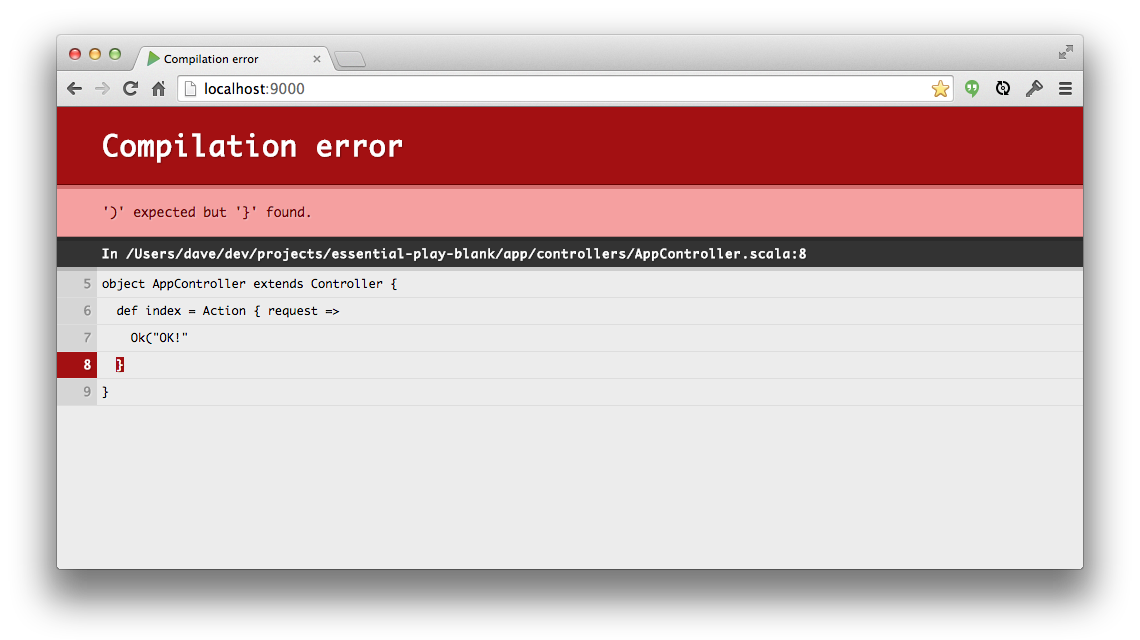
\includegraphics{src/pages/basics/compile-error.png}
\caption{Internal error: Play's compilation error 500 page}
\end{figure}

While this behaviour is useful, we should be aware of two drawbacks:

\begin{enumerate}
\def\labelenumi{\arabic{enumi}.}
\item
  The web page only reports the \emph{first} error from the SBT console.
  A single typo in Scala code can create several compiler errors, so we
  often have to look at the complete output from SBT to trace down a
  bug.
\item
  When we use \texttt{sbt run}, Play only recompiles our code when we
  refresh the web page. This sometimes slows down development because we
  have to constantly switch back and forth between editor and browser.

  We can write and debug code faster if we use SBT's \emph{continuous
  compilation} mode instead of \texttt{sbt run}. To start continuous
  compilation, type \texttt{\textasciitilde{}compile} on the SBT
  console:

\begin{verbatim}
[hello-world] $ ~compile
[success] Total time: 0 s, completed 11-Oct-2014 11:46:28
1. Waiting for source changes... (press enter to interrupt)
\end{verbatim}

  In continuous compilation mode, SBT recompiles our code every time we
  change a file. However, we have to go back to \texttt{sbt run} to see
  the changes in a browser.
\end{enumerate}

\subsection{Runtime Errors}\label{runtime-errors}

If our code compiles but fails at runtime, we get a similar error page
that points to the source of the exception. The exception is reported on
the SBT console as well as on the page:

\begin{figure}[htbp]
\centering
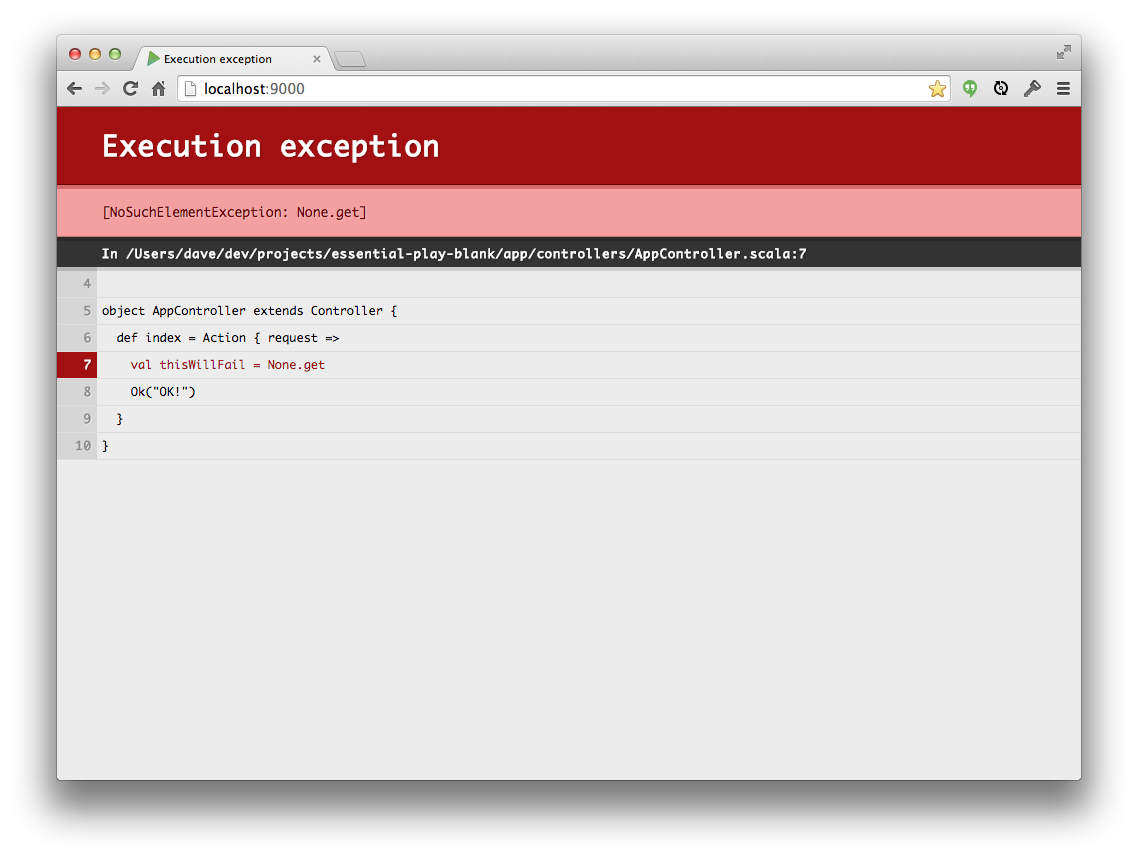
\includegraphics{src/pages/basics/internal-error.png}
\caption{Internal error: Play's default error 500 page}
\end{figure}

\subsection{Routing Errors}\label{routing-errors}

Play generates a 404 page if it can't find an appropriate route for an
incoming request. This error \emph{doesn't} appear on the console:

\begin{figure}[htbp]
\centering
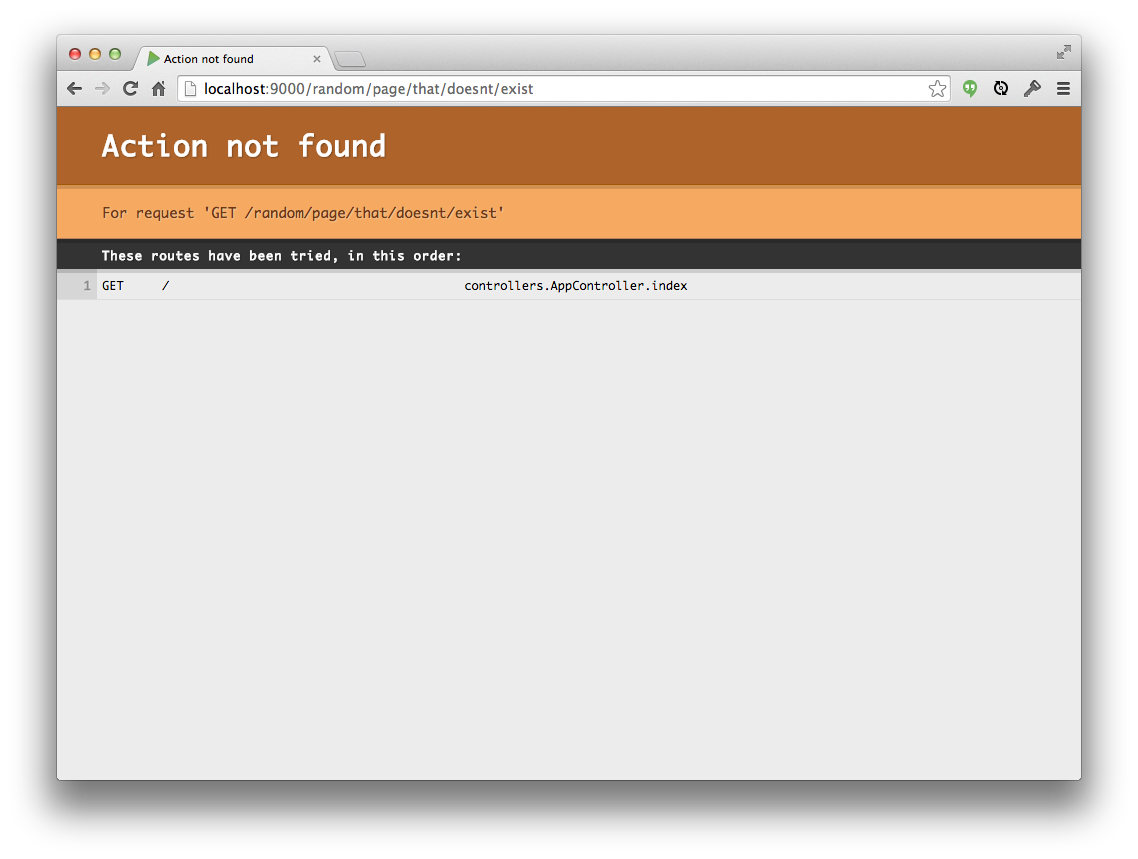
\includegraphics{src/pages/basics/not-found-error.png}
\caption{Not found: Play's 404 routing error page}
\end{figure}

If Play finds a route but can't parse the parameters from the path and
query string, it issues a similar-looking 400 response:

\begin{figure}[htbp]
\centering
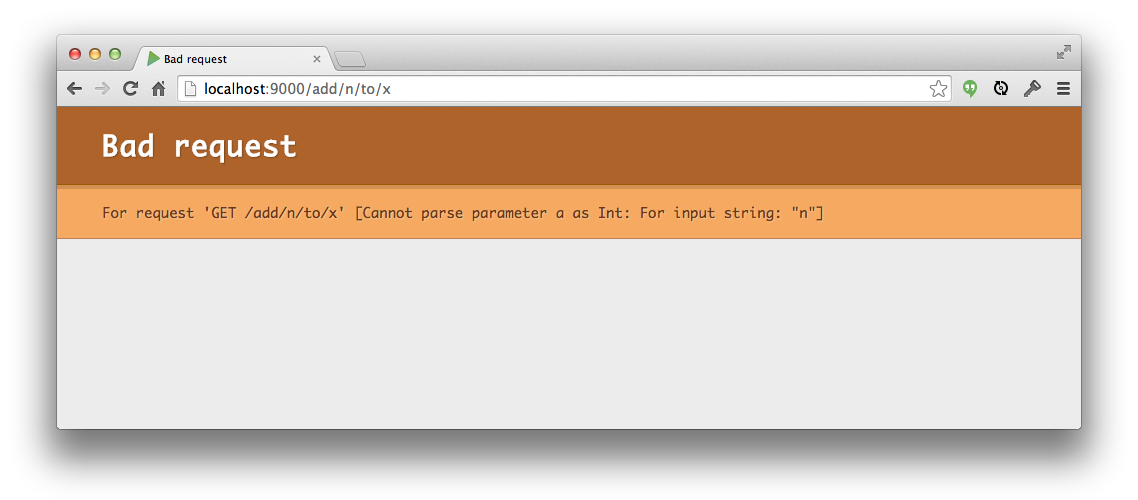
\includegraphics{src/pages/basics/bad-request-error.png}
\caption{Bad request: Play's 400 routing error page}
\end{figure}

\subsection{Take Home Points}\label{take-home-points-4}

Play ships with a default 500 error page out of the box. It gives us
nice error messages for compile errors and exceptions during
development. Similarly, Play provides default 404 and 400 pages for
routing errors.

These error messages are useful during development, but we should
remember to disable it before we put code into production. We will see
this next chapter when we create our own HTML and learn how to handle
form data.

\hyperdef{}{chapter-html}{\chapter{HTML and Forms}\label{chapter-html}}

In the last chapter we saw how to receive HTTP requests and send
responses. However, we dealt exclusively with content of type
\texttt{text/plain}. In this chapter we will generate HTML content using
Play's templating language, \emph{Twirl}. We will also learn how to
create HTML forms and parse and validate submitted form data.

\section{Twirl Templates}\label{twirl-templates}

Play uses a PHP-like templating language called \emph{Twirl} to generate
HTML. Templates are compiled to function objects that can be called
directly from regular Scala code. In this section we will look at the
Twirl syntax and compilation process.

\subsection{A First Template}\label{a-first-template}

Twirl templates resemble plain HTML with embedded Scala-like dynamic
expressions:

\begin{Shaded}
\begin{Highlighting}[]
\CommentTok{<!-- In app/views/helloWorld.scala.html -->}
\NormalTok{@(name: String)}

\KeywordTok{<html>}
  \KeywordTok{<head>}
    \KeywordTok{<title>}\NormalTok{Hello @name}\KeywordTok{</title>}
  \KeywordTok{</head>}

  \KeywordTok{<body>}
    \KeywordTok{<p>}\NormalTok{Hello there, @name.toUpperCase!}\KeywordTok{</p>}
  \KeywordTok{</body>}
\KeywordTok{</html>}
\end{Highlighting}
\end{Shaded}

The first line of the template describes its \emph{parameters}. The
format is an \texttt{@} sign followed by one or more Scala parameter
lists. The rest of the template consists of plain HTML content with
dynamic \texttt{@expressions}. The expression syntax is based on Scala
code with a couple of Twirl-specific tweaks -- read on for details:

\begin{Shaded}
\begin{Highlighting}[]
\KeywordTok{package} \NormalTok{views.}\FunctionTok{html}

\KeywordTok{import} \NormalTok{play.}\FunctionTok{twirl}\NormalTok{.}\FunctionTok{api}\NormalTok{.}\FunctionTok{Html}

\KeywordTok{object} \NormalTok{helloWorld \{}
  \KeywordTok{def} \FunctionTok{apply}\NormalTok{(name: String): Html = \{}
    \CommentTok{// ...}
  \NormalTok{\}}
\NormalTok{\}}
\end{Highlighting}
\end{Shaded}

\subsection{File Names and Compiled
Names}\label{file-names-and-compiled-names}

We should place templates in the \texttt{app/views} folder and give them
\texttt{.scala.html} filename extensions. Their compiled forms are named
based on our filenames and placed in the \texttt{views.html} package.
Here are some examples:

\textbar{}---------------------------------------------------------------------------------\textbar{}
\textbar{} Template file name \textbar{} Scala object name \textbar{}
\textbar{}---------------------------------------------------------------------------------\textbar{}
\textbar{} \texttt{views/helloWorld.scala.html} \textbar{}
\texttt{views.html.helloWorld} \textbar{} \textbar{}
\texttt{views/user/loginForm.scala.html} \textbar{}
\texttt{views.html.user.loginForm} \textbar{} \textbar{}
\texttt{views/foo/bar/baz.scala.html} \textbar{}
\texttt{views.html.foo.bar.baz} \textbar{}
\textbar{}=================================================================================\textbar{}
\{: .table .table-bordered .table-responsive \}

Templates return objects of type
\href{https://github.com/playframework/twirl/blob/master/api/src/main/scala/play/twirl/api/Formats.scala}{play.twirl.api.Html}.
Play knows how to serialize \texttt{Html} values in the
\texttt{Results}. This makes it easy to use templates in our
\texttt{Actions}:

\begin{Shaded}
\begin{Highlighting}[]
\KeywordTok{def} \NormalTok{index = Action \{ request =>}
  \FunctionTok{Ok}\NormalTok{(views.}\FunctionTok{html}\NormalTok{.}\FunctionTok{helloWorld}\NormalTok{(}\StringTok{"Dave"}\NormalTok{))}
\NormalTok{\}}
\end{Highlighting}
\end{Shaded}

\begin{WarningCallout}

\emph{Non-HTML Templates}

Twirl templates can also be used to generate XML, Javascript, and plain
text responses. The folders, packages, and return types vary, but
otherwise these templates are identical to the HTML templates discussed
here:

\textbar{}-----------------------------------------------------------------------------------------------------\textbar{}
\textbar{} Template type \textbar{} Source folder \textbar{} Filename
extension \textbar{} Compiled package \textbar{} Return type \textbar{}
\textbar{}-----------------------------------------------------------------------------------------------------\textbar{}
\textbar{} HTML \textbar{} \texttt{app/views} \textbar{}
\texttt{.scala.html} \textbar{} \texttt{views.html} \textbar{}
\href{https://github.com/playframework/twirl/blob/master/api/src/main/scala/play/twirl/api/Formats.scala}{play.twirl.api.Html}
\textbar{} \textbar{} XML \textbar{} \texttt{app/views} \textbar{}
\texttt{.scala.xml} \textbar{} \texttt{views.xml} \textbar{}
\href{https://github.com/playframework/twirl/blob/master/api/src/main/scala/play/twirl/api/Formats.scala}{play.twirl.api.Xml}
\textbar{} \textbar{} Javascript \textbar{} \texttt{app/views}
\textbar{} \texttt{.scala.js} \textbar{} \texttt{views.js} \textbar{}
\href{https://github.com/playframework/twirl/blob/master/api/src/main/scala/play/twirl/api/Formats.scala}{play.twirl.api.Txt}
\textbar{} \textbar{} Plain text \textbar{} \texttt{app/views}
\textbar{} \texttt{.scala.txt} \textbar{} \texttt{views.txt} \textbar{}
\href{https://github.com/playframework/twirl/blob/master/api/src/main/scala/play/twirl/api/Formats.scala}{play.twirl.api.JavaScript}
\textbar{}
\textbar{}=====================================================================================================\textbar{}
\{: .table .table-bordered .table-responsive \}

\end{WarningCallout}

\subsection{Parameters and
expressions}\label{parameters-and-expressions}

Twirl templates can have any number of parameters of arbitrary types.
They also support features such as default parameter values and
multiple/implicit parameter lists:

\begin{Shaded}
\begin{Highlighting}[]
\CommentTok{<!-- user.scala.html -->}
\NormalTok{@(user: User, showEmail: Boolean = true)(implicit obfuscate: EmailObfuscator)}

\KeywordTok{<ul>}
  \KeywordTok{<li>}\NormalTok{@user.name}\KeywordTok{</li>}
  \NormalTok{@if(showEmail) \{}
    \KeywordTok{<li>}\NormalTok{@obfuscate(user.email)}\KeywordTok{</li>}
  \NormalTok{\}}
\KeywordTok{</ul>}
\end{Highlighting}
\end{Shaded}

The template body is compiled to a single Scala expression that appends
all the static and dynamic parts to a single \texttt{Html} object. Twirl
uses runtime pattern matching to convert embedded expressions to HTML.
All expressions are escaped to prevent code injection vulnerabilities:

\begin{itemize}
\itemsep1pt\parskip0pt\parsep0pt
\item
  simple values such as \texttt{Strings}, \texttt{Ints} and
  \texttt{Booleans} yield representative text;
\item
  \texttt{Seqs}, \texttt{Arrays} and Java collections yield content for
  every item (no delimiter);
\item
  \texttt{Optional} values yield text content when full and no content
  when empty;
\item
  \texttt{Unit} values yield no content.
\end{itemize}

Twirl embedded expression syntax is inspired by Scala syntax. Here is a
brief synopsis -- for more information see Play's
\href{https://www.playframework.com/documentation/2.3.x/ScalaTemplates}{documentation
on template syntax}.

\subsubsection{Simple Expressions}\label{simple-expressions}

Dynamic expressions are prefixed using the \texttt{@} character. We
don't need to indicate the end of an expression -- Twirl attempts to
automatically work out where the Scala code ends and HTML begins:

\begin{multicols}{2}

\begin{Shaded}
\begin{Highlighting}[]
\KeywordTok{<p>}\NormalTok{Hello, @"Dave".toUpperCase!}\KeywordTok{</p>}
\end{Highlighting}
\end{Shaded}

\columnbreak

\begin{Shaded}
\begin{Highlighting}[]
\KeywordTok{<p>}\NormalTok{Hello, DAVE!}\KeywordTok{</p>}
\end{Highlighting}
\end{Shaded}

\end{multicols}

\subsubsection{Wrapped Expressions}\label{wrapped-expressions}

Twirl occasionally has difficulty determining where dynamic code ends
and static content begins. If this is a problem we can use parentheses
or braces to delimit the dynamic content:

\begin{multicols}{2}

\begin{Shaded}
\begin{Highlighting}[]
\KeywordTok{<p>}\NormalTok{The first answer is @(1 + 2).}\KeywordTok{</p>}

\KeywordTok{<p>}\NormalTok{The second answer is @\{}
  \NormalTok{val a = 3}
  \NormalTok{val b = 4}
  \NormalTok{a + b}
\NormalTok{\}.}\KeywordTok{</p>}
\end{Highlighting}
\end{Shaded}

\columnbreak

\begin{Shaded}
\begin{Highlighting}[]
\KeywordTok{<p>}\NormalTok{The first answer is 3.}\KeywordTok{</p>}

\KeywordTok{<p>}\NormalTok{The second answer is 7.}\KeywordTok{</p>}
\end{Highlighting}
\end{Shaded}

\end{multicols}

\subsubsection{Method Calls}\label{method-calls}

Method calls can be written as usual. Twirl treats parameters between
parentheses as Scala:

\begin{multicols}{2}

\begin{Shaded}
\begin{Highlighting}[]
\KeywordTok{<p>}\NormalTok{The maximum is @math.max(1, 2, 3).}\KeywordTok{</p>}
\end{Highlighting}
\end{Shaded}

\columnbreak

\begin{Shaded}
\begin{Highlighting}[]
\KeywordTok{<p>}\NormalTok{The maximum is 3.}\KeywordTok{</p>}
\end{Highlighting}
\end{Shaded}

\end{multicols}

Methods of one parameter can be called using braces instead. Twirl
parses the parameter between the braces as HTML:

\begin{multicols}{2}

\begin{Shaded}
\begin{Highlighting}[]
\KeywordTok{<ul>}
  \NormalTok{@(1 to 3).map \{ item =>}
    \KeywordTok{<li>}\NormalTok{Item @item}\KeywordTok{</li>}
  \NormalTok{\}}
\KeywordTok{</ul>}
\end{Highlighting}
\end{Shaded}

\columnbreak

\begin{Shaded}
\begin{Highlighting}[]
\KeywordTok{<ul>}
  \KeywordTok{<li>}\NormalTok{Item 1}\KeywordTok{</li>}
  \KeywordTok{<li>}\NormalTok{Item 2}\KeywordTok{</li>}
  \KeywordTok{<li>}\NormalTok{Item 3}\KeywordTok{</li>}
\KeywordTok{</ul>}
\end{Highlighting}
\end{Shaded}

\end{multicols}

\subsubsection{Conditionals}\label{conditionals}

If we delimit the true and false arms using braces, Twirl treats them as
HTML. Otherwise they are treated as Scala code:

\begin{multicols}{2}

\begin{Shaded}
\begin{Highlighting}[]
\CommentTok{<!-- a = 1000, b = 2000 -->}
\KeywordTok{<p>}
  \NormalTok{@if(1 > 2) \{}
    \KeywordTok{<em>}\NormalTok{Help! All of maths is wrong!}\KeywordTok{</em>}
  \NormalTok{\} else \{}
    \KeywordTok{<em>}\NormalTok{Phew! Looks like we're ok.}\KeywordTok{</em>}
  \NormalTok{\}}
\KeywordTok{</p>}
\end{Highlighting}
\end{Shaded}

\columnbreak

\begin{Shaded}
\begin{Highlighting}[]
\KeywordTok{<p><em>}\NormalTok{Phew! Looks like we're ok.}\KeywordTok{</em></p>}
\end{Highlighting}
\end{Shaded}

\end{multicols}

If we omit the false arm of a Scala conditional, it evaluates to
\texttt{Unit}. Twirl renders this as empty content:

\begin{multicols}{2}

\begin{Shaded}
\begin{Highlighting}[]
\KeywordTok{<p>}\NormalTok{Everything is @if(false) \{ NOT \} ok.}\KeywordTok{</p>}
\end{Highlighting}
\end{Shaded}

\columnbreak

\begin{Shaded}
\begin{Highlighting}[]
\KeywordTok{<p>}\NormalTok{Eerything is  ok.}\KeywordTok{</p>}
\end{Highlighting}
\end{Shaded}

\end{multicols}

\subsubsection{Match Expressions}\label{match-expressions}

If we wrap the right-hand-sides of case clauses in braces, Twirl treats
them as HTML content. Otherwise they are treated as Scala code:

\begin{multicols}{2}

\begin{Shaded}
\begin{Highlighting}[]
\KeywordTok{<p>}
  \NormalTok{@List("foo", "bar", "baz") match \{}
    \NormalTok{case Nil => "the list is empty"}
    \NormalTok{case a :: b => \{}
      \KeywordTok{<em>}\NormalTok{the list has many elements:}
      \NormalTok{@a, and @(b.lenth) others}\KeywordTok{</em>}
    \NormalTok{\}}
  \NormalTok{\}}
\KeywordTok{</p>}
\end{Highlighting}
\end{Shaded}

\columnbreak

\begin{Shaded}
\begin{Highlighting}[]
\KeywordTok{<p>}
  \KeywordTok{<em>}\NormalTok{the list has mane elements:}
  \NormalTok{foo, and 2 others}\KeywordTok{</em>}
\KeywordTok{</p>}
\end{Highlighting}
\end{Shaded}

\end{multicols}

\subsubsection{For-Comprehensions}\label{for-comprehensions}

For-comprehensions are supported without the \texttt{yield} keyword,
which is implicitly assumed in Twirl syntax:

\begin{multicols}{2}

\begin{Shaded}
\begin{Highlighting}[]
\KeywordTok{<ul>}
  \NormalTok{@for(item }\ErrorTok{<}\NormalTok{- 1 to 3) \{}
    \KeywordTok{<li>}\NormalTok{Item @item}\KeywordTok{</li>}
  \NormalTok{\}}
\KeywordTok{</ul>}
\end{Highlighting}
\end{Shaded}

\columnbreak

\begin{Shaded}
\begin{Highlighting}[]
\KeywordTok{<ul>}
  \KeywordTok{<li>}\NormalTok{Item 1}\KeywordTok{</li>}
  \KeywordTok{<li>}\NormalTok{Item 2}\KeywordTok{</li>}
  \KeywordTok{<li>}\NormalTok{Item 3}\KeywordTok{</li>}
\KeywordTok{</ul>}
\end{Highlighting}
\end{Shaded}

\end{multicols}

\subsubsection{Pre-Defined Helpers}\label{pre-defined-helpers}

Twirl provides a \texttt{defining} method as a means of aliasing complex
Scala expressions as single identifiers:

\begin{multicols}{2}

\begin{Shaded}
\begin{Highlighting}[]
\KeywordTok{<p>}
  \NormalTok{@defining(1 + 2 + 3 + 4 + 5) \{ sum =>}
    \NormalTok{The answer is @sum.}
  \NormalTok{\}}
\KeywordTok{</p>}
\end{Highlighting}
\end{Shaded}

\columnbreak

\begin{Shaded}
\begin{Highlighting}[]
\KeywordTok{<p>}
  \NormalTok{The answer is 15.}
\KeywordTok{</p>}
\end{Highlighting}
\end{Shaded}

\end{multicols}

Play also provides a variety of pre-defined templates in the
\href{https://www.playframework.com/documentation/2.3.x/api/scala/index.html\#views.html.helper.package}{views.html.helper}
package. We will discuss some of these in the next section.

\subsection{Nesting Templates}\label{nesting-templates}

Because Twirl templates compile to Scala functions, we can call one
template from another. We can also pass \texttt{Html} content from one
template to another to create wrapper-style constructions:

\begin{multicols}{2}

\begin{Shaded}
\begin{Highlighting}[]
\CommentTok{<!-- In app/views/main.scala.html -->}
\NormalTok{@hello("Dave")}

\CommentTok{<!-- In app/views/hello.scala.html -->}
\NormalTok{@(name: String)}

\NormalTok{@layout("Hello " + name) \{}
  \KeywordTok{<p>}\NormalTok{Hello there, @name.}\KeywordTok{</p>}
\NormalTok{\}}

\CommentTok{<!-- In app/views/layout.scala.html -->}
\NormalTok{@(title: String)(body: Html)}

\KeywordTok{<html>}
  \KeywordTok{<head>}
    \KeywordTok{<title>}\NormalTok{@title}\KeywordTok{</title>}
  \KeywordTok{</head>}
  \KeywordTok{<body>}
    \NormalTok{@body}
  \KeywordTok{</body>}
\KeywordTok{</html>}
\end{Highlighting}
\end{Shaded}

\columnbreak

\begin{Shaded}
\begin{Highlighting}[]
\KeywordTok{<html>}
  \KeywordTok{<head>}
    \KeywordTok{<title>}\NormalTok{Hello Dave}\KeywordTok{</title>}
  \KeywordTok{</head>}
  \KeywordTok{<body>}
    \KeywordTok{<p>}\NormalTok{Hello there, Dave.}\KeywordTok{</p>}
  \KeywordTok{</body>}
\KeywordTok{</html>}
\end{Highlighting}
\end{Shaded}

\end{multicols}

\subsection{Take Home Points}\label{take-home-points-5}

We create HTML in Play using a templating language called \emph{Twirl}.

We place Twirl templates in the \texttt{app/views} folder and give them
the extension \texttt{.scala.html}.

Templates are compiled to singleton Scala functions in the
\texttt{views.html} package.

Template functions accept whatever parameters we define and return
instances of
\href{https://github.com/playframework/twirl/blob/master/api/src/main/scala/play/twirl/api/Formats.scala}{play.twirl.api.Html}.
Play understands how to serialize \texttt{Html} objects as content
within \texttt{Results}. It even sets the \texttt{Content-Type} for us.

\end{document}
